\documentclass[11pt]{article}
\pdfoutput=1
\usepackage{jhepmod}
\usepackage{booktabs}
\usepackage[english]{babel}
\usepackage{amsmath,amssymb,amsbsy,amstext, amsthm, simplewick}
\usepackage{graphicx}
\usepackage{amsfonts}
\usepackage{mathtools}
\usepackage{amssymb}
\usepackage{upgreek}
\usepackage{listings}
\usepackage{exscale,relsize}
\usepackage[makeroom]{cancel}
\usepackage{soul}
\usepackage[utf8]{inputenc}
\RequirePackage{color}
\usepackage{amsopn, amstext, wasysym}
\usepackage{colonequals}
\usepackage{rotating}
\usepackage{multirow}
\usepackage{xspace}
\usepackage{datetime}
\usepackage[framemethod=tikz]{mdframed}
\newcommand{\db}[1]{\textcolor{green2}{(DB: #1)}}
\newcommand{\dg}[1]{\textcolor{darkgreen}{(DG: #1)}}
\newcommand{\DB}[1]{\textcolor{red}{ #1}}
\newcommand{\rp}[1]{\textcolor{blue}{#1}}
\usepackage[T1]{fontenc}
\usepackage{graphicx,scalerel}
\newmdenv[innerlinewidth=0.5pt, roundcorner=4pt,linecolor=mycolor,innerleftmargin=6pt,
innerrightmargin=6pt,innertopmargin=6pt,innerbottommargin=6pt]{mybox}

\newmdenv[innerlinewidth=0.5pt, roundcorner=4pt,linecolor=mauve,innerleftmargin=6pt,
innerrightmargin=6pt,innertopmargin=6pt,innerbottommargin=6pt]{mybox2}

\usetikzlibrary{backgrounds,fit,decorations.pathreplacing,calc}


\renewcommand{\baselinestretch}{1.14}


\definecolor{navyblue}{rgb}{0.0, 0.0, 0.9}
\definecolor{rindou1}{rgb}{0.4431,0.2862,0.7960}
\definecolor{rindou2}{rgb}{0.078,0.1215,0.4392}
\definecolor{BrickRed}{rgb}{0.0, 0.53, 0.74}
\definecolor{BlueNCS}{rgb}{0.0, 0.53, 0.74}
\definecolor{mycolor}{rgb}{0.122, 0.435, 0.698}
\definecolor{mycolor2}{rgb}{0.02, 0.435, 0.698}
\definecolor{dkgreen}{rgb}{0,0.6,0}
\definecolor{gray}{rgb}{0.5,0.5,0.5}
\definecolor{mauve}{rgb}{0.58,0.33,0.82}
\definecolor{green2}{cmyk}{0, 1, 0.5, 0}
\definecolor{lightgreen}{cmyk}{0.2, 0, 0.2, 0.2}
\definecolor{lightgray}{cmyk}{0.1,0.2,0,0.1}
\definecolor{lightgray2}{cmyk}{0.4,0.4,0,0.8}
\definecolor{black}{cmyk}{1.0,1.0,1.0,1.0}
\definecolor{celadon}{rgb}{0.67,0.88,0.69}

\lstset{frame=none,
	language=Python,
	aboveskip=1mm,
	belowskip=1mm,
	numbers=left,
	showstringspaces=false,
	columns=flexible,
	basicstyle={\ttfamily\footnotesize},
	numberstyle=\tiny\color{black},
	keywordstyle=\color{blue},
	commentstyle=\color{gray},
	stringstyle=\color{mycolor2},
	breaklines=true,
	breakatwhitespace=true,
	tabsize=3, 
	keepspaces=true
}

\newcommand{\TODO}[1]{\textcolor{red}{\textbf{#1}}}


\usepackage{amsthm}
\usepackage{upgreek}
\usepackage{slashed}
\usepackage{verbatim} 
\usepackage{scalerel}
\usepackage{lmodern}
%\usepackage[x11names]{xcolor}
\usepackage{framed}
%\colorlet{shadecolor}{LavenderBlush2} 
%\colorlet{framecolor}{Red1}
\usepackage{lipsum}
\usepackage{xcolor}
\usepackage{mathrsfs}
\usetikzlibrary{arrows}
\usepackage{colortbl}
\usepackage[framemethod=tikz]{mdframed}



\newenvironment{frshaded}{%
	\def\FrameCommand{\fboxrule=\FrameRule\fboxsep=\FrameSep \fcolorbox{framecolor}{shadecolor}}%
	\MakeFramed {\FrameRestore}}%
{\endMakeFramed}

\newenvironment{frshaded*}{%
	\def\FrameCommand{\fboxrule=\FrameRule\fboxsep=\FrameSep \fcolorbox{framecolor}{shadecolor}}%
	\MakeFramed {\advance\hsize-\width \FrameRestore}}%
{\endMakeFramed}

% Shortcuts
\def\figheight{8.9 cm}
\usepackage{pgf,tikz}
\usepackage{mathrsfs}
\usetikzlibrary{arrows}
\usepackage{placeins}
\usepackage{pgf,tikz}
\usepackage{mathtools}
\usetikzlibrary{arrows.meta}



\usepackage[utf8]{inputenc}
\usepackage[english]{babel}
\usepackage{graphicx,tipa}
\usepackage{csquotes}
\usepackage{amsmath}
\usepackage{amssymb}
\usepackage{xcolor}
\usepackage{color,wasysym}
\usepackage{bbold}
\usepackage[abs]{overpic}
\usepackage[T1]{fontenc}
\usepackage{hyperref}
\usepackage{cancel}
%\usepackage{qcircuit}
\usepackage[braket, qm]{qcircuit}
% Learn from: https://github.com/CQuIC/qcircuit/blob/master/Qtutorial.tex


%\usetikzlibrary{quantikz}


\definecolor{redred}{HTML}{D53E4F}
\newcommand{\danger}[1]{{\color{red} #1}}

\definecolor{blueblue}{HTML}{1B57B6}
\newcommand{\blue}[1]{{\color{blueblue} #1}}


\newcommand{\kp}{\ket{\psi}}
\newcommand{\bp}{\bra{\psi}}
\newcommand{\Id}{{\mathbb 1}}
\newcommand{\eS}{\mathcal{S}}
\newcommand{\mb}{\bar{m}}
\newcommand{\tm}{(\text{th})}
\newcommand{\eM}{\mathcal{M}}
\newcommand{\eN}{\mathcal{N}}
\newcommand{\eL}{\mathcal{L}}
\newcommand{\Cor}{\mathfrak{C}}
\newcommand{\Dsla}{\cancel{\mathcal{D}}}
\newcommand{\Asla}{\cancel{\mathcal{A}}}
\newcommand{\sigsla}{\cancel{\sigma}}
\newcommand{\gspa}{\mathfrak{S}}
\newcommand{\trace}{\mbox{Tr}}
\newcommand{\ie}{i.e.,~}
\newcommand{\eg}{e.g.~}
\newcommand{\T}{\texttt}
\newcommand{\PAD}{\textsc{Pandas}}
\newcommand{\QIS}{\textsc{Qiskit}}

% Make Orcid icon
\usepackage{tikz,xcolor,hyperref}
\definecolor{lime}{HTML}{A6CE39}
\DeclareRobustCommand{\orcidicon}{%
	
\begin{tikzpicture}
	\draw[lime, fill=lime] (0,0) 
	circle [radius=0.16] 
	node[white] {{\fontfamily{qag}\selectfont \tiny ID}};	\draw[white, fill=white] (-0.0625,0.095) 
	circle [radius=0.007];	\end{tikzpicture}
	\hspace{-2mm}}
\foreach \x in {A,...,Z}{%
	\expandafter\xdef\csname orcid\x\endcsname{\noexpand\href{https://orcid.org/\csname orcidauthor\x\endcsname}{\noexpand\orcidicon}}
}
\newcommand{\orcidauthorA}{0000-0003-2933-0102} %ORCID number for the author


\newcommand{\filling}{f_M}
\newcommand{\len}{\text{L}}
\usepackage{environ}
\usepackage{varwidth}
%\usepackage{showframe}
\newlength{\TheoremWidthTweak}%

\NewEnviron{short-shaded}[1][]{%
	\setlength{\TheoremWidthTweak}{\dimexpr%
		+\mdflength{innerleftmargin}
		+\mdflength{innerrightmargin}
		+\mdflength{leftmargin}
		+\mdflength{rightmargin}
	}%
	\savebox0{%
		\begin{varwidth}{\dimexpr\linewidth-\TheoremWidthTweak\relax}%
			\BODY
		\end{varwidth}%
	}%
	\begin{mdframed}[backgroundcolor=lightgray,userdefinedwidth=\dimexpr\wd0+\TheoremWidthTweak\relax, #1]
		\usebox0
	\end{mdframed}
}

\begin{document}
	\begin{titlepage}
		\setcounter{page}{1} \baselineskip=15.5pt \thispagestyle{empty}
		\bigskip\
		\vspace{1cm}
		\begin{center}
			{\fontsize{19}{38}\textsc{Notes on Machine Learning}}  %- \large{Beginner's Guide}}}
		\end{center}
		\vspace{0.2cm}
		\begin{center}
			{\fontsize{12}{30}\selectfont Raghav G.~Jha\orcidA{}\,\footnote{\texttt{raghav.govind.jha@gmail.com}}}
		\end{center}
		
		
		\begin{center}
			\vskip 7pt
			\textsl{Thomas Jefferson National Accelerator Facility, Newport News, VA 23606, USA\\
			Perimeter Institute for Theoretical Physics, Waterloo, Ontario N2L 2Y5\\
				}
			\vskip 6pt
		\end{center}
		
		\vspace{2.6cm}
		\hrule \vspace{0.2cm}
		\noindent {\sffamily \bfseries Abstract}{ \\[0.1cm]
These notes cover some basic ideas and theory behind the field of machine learning. These notes are by no means 
even close to being exhaustive and simply meant for quick reference and interview preparation. Partly inspired by the 
amazing 100-page textbook.\footnote{The Hundred-Page Machine Learning Book. by Andriy Burkov, Quebec City, Canada, 2019}}
\vspace{0.5cm}
\hrule

\vspace{0.5cm}		
		\tableofcontents
		\vspace{0.6cm}
	\end{titlepage}
	
	
	\section{introduction}
	
	it is no exagerration to say that all aspects of human life is related to data. What we buy, what we buy online and many others
	are all data-driven and uses machine learning (ML) methods. What movies are recommended to you on Netflix or what Amazon
	recommends you to buy in bundle are all determined by various algorithms of ML. The pricing of airline tickets and the web history 
	or what links you visit all determines what you are being shown online and how much you pay. 
	
	These notes are a brief introduction to the fundamentals and methods used in machine learning. Usually, ML is 
	classified into three parts: Supervised, Unsupervised, Reinforcement learning. The canvas of ML is shown in Fig.~\ref{fig:EXP}. 
	
	
	
	
	\newpage
	\section{Some famous ML algorithms}
	
	
	

\begin{figure}
\centering 
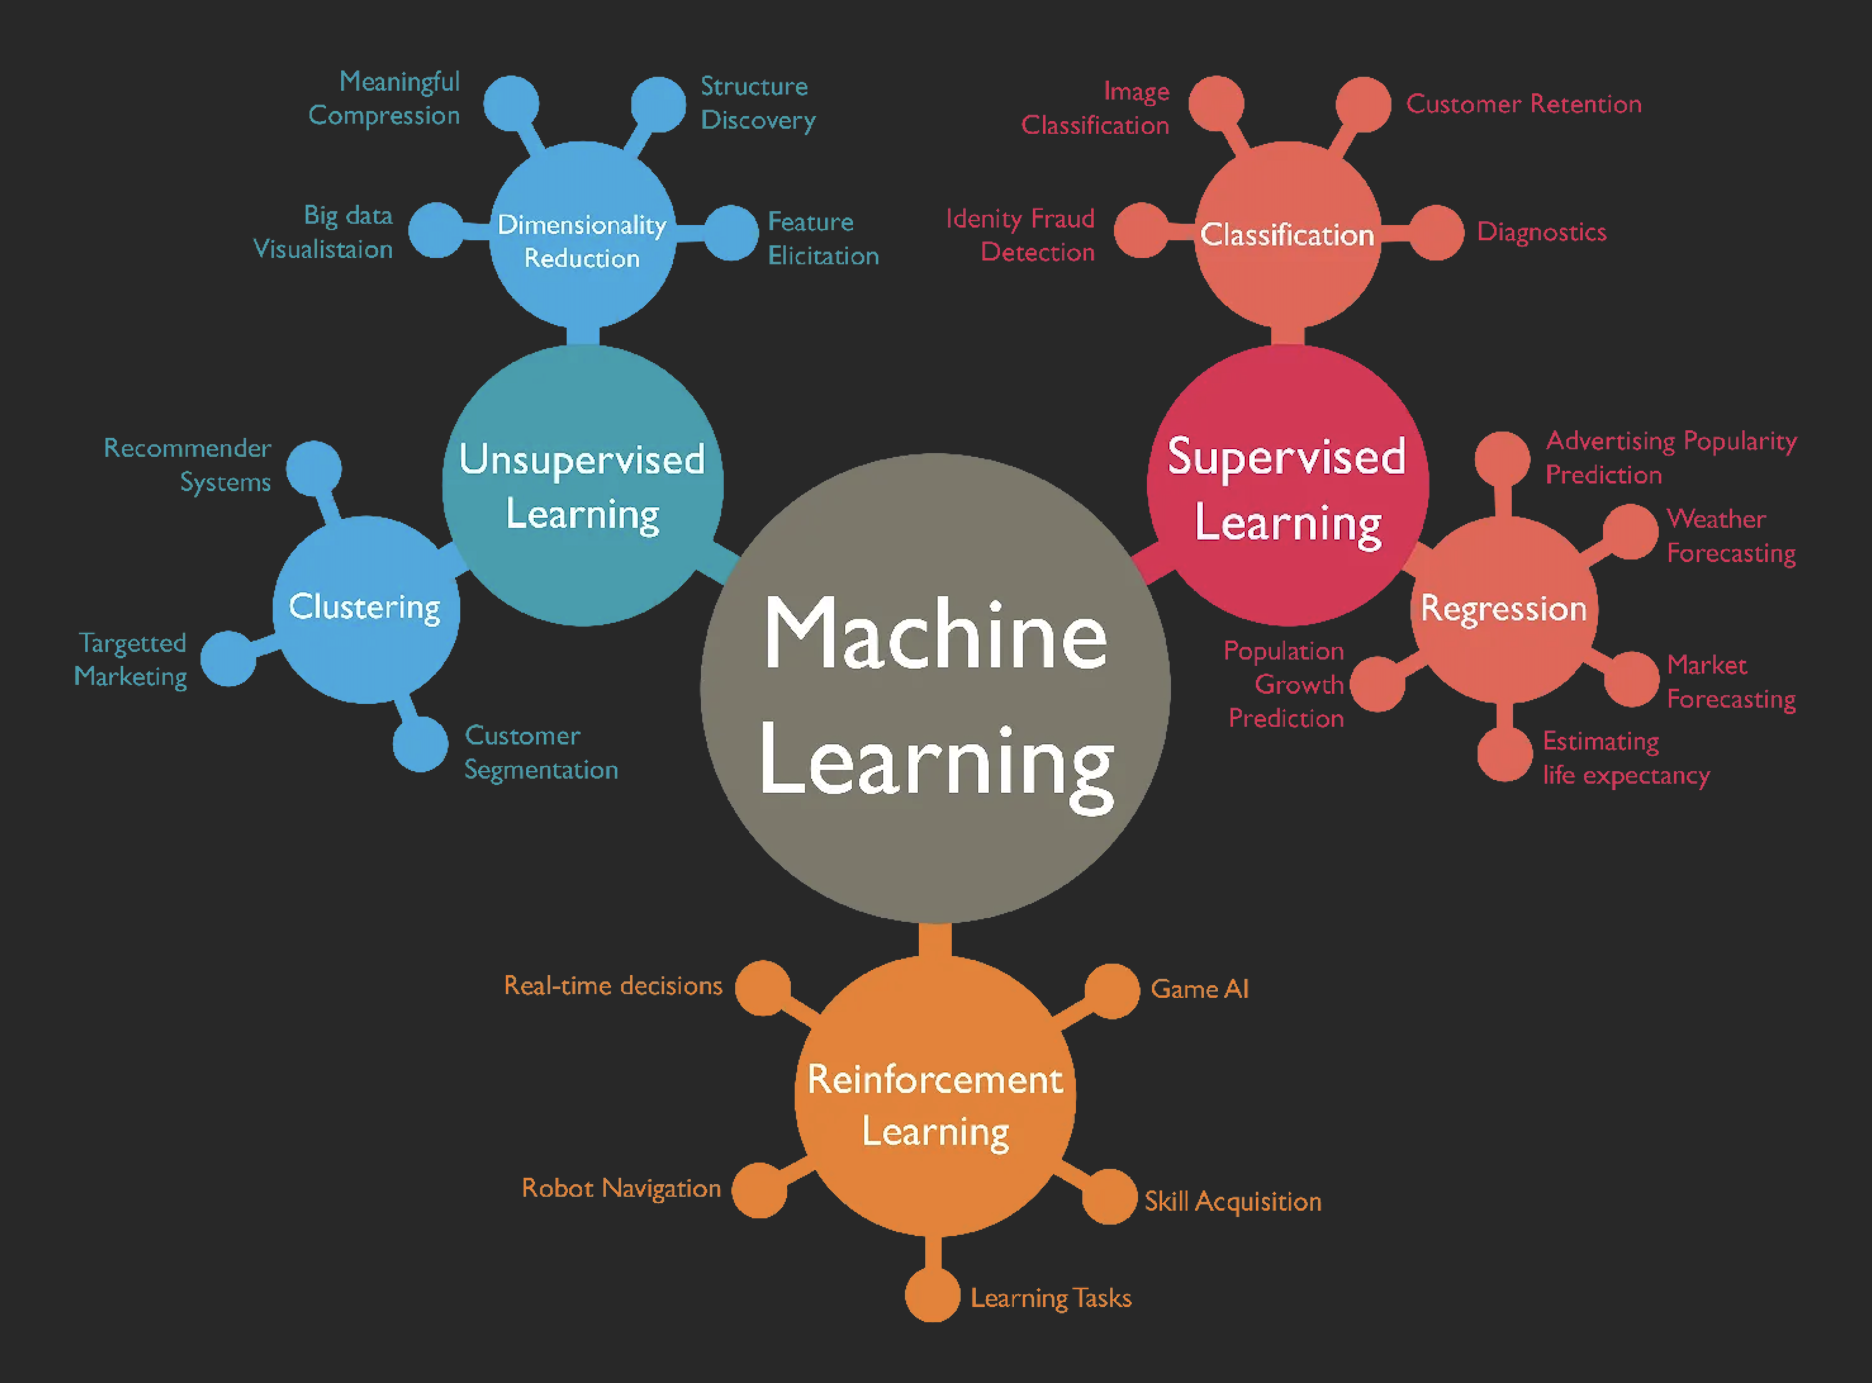
\includegraphics[width=0.65\textwidth]{cartoonML.png}
\caption{\label{fig:EXP}A cartoon showing the landscape of machine learning.}
\end{figure}
	
	
Some popular ML algorithms are: 

\begin{itemize}
\item Linear regression: This gives a relationship between input $x$ and an output variable $y$, also referred to as independent and dependent variables. 
Consider an example where you are required to arrange a few plastic boxes of different sizes on separate shelves based on their corresponding weights.
The task is to be completed without manually weighing the boxes. Instead, you need to guess the weight just by observing the height, dimensions, and sizes of the box. 
In short, the entire task is driven based on visual analysis. Thus, you have to use a combination of visible variables to make the 
final arrangement on the shelves. Linear regression in machine learning is of a similar kind, where the relationship between independent and dependent variables is established 
by fitting them to a regression line. This line has a mathematical representation given by the linear equation $y = wx + c$, where $y$ represents the dependent variable, 
$w$ = slope, $x$ = independent variable, and $b$ = intercept. We need to find the best fit by minimizing the errors using Ordinary Least Squares (OLS) as:
\begin{equation}
\text{Min.} \sum_{i=1}^{N} (y_{i} - w_{i} x_{i})
\end{equation}
\item Logistic regression: The dependent variable is of binary type (dichotomous) in logistic regression. This type of regression analysis describes data and explains the relationship between one dichotomous variable and one or more independent variables.
Logistic regression is used in predictive analysis where pertinent data predict an event probability to a logit function. Thus, it is also called logit regression.
Mathematically, logistic regression is represented by the equation:
\begin{equation}
y = \exp(b_{0} + b_{1}x)/1 + \exp(b_{0} + b_{1}x))
\end{equation}
where $x$ = input value, $y$ = predicted output, $b_0$ = bias or intercept term, $b_1$ = coefficient for input $x$.
Logistic regression could be used to predict whether a particular team will win (1) a tournament or not (0), 
or whether a lockdown will be imposed (1) due to rising COVID-19 cases or not (0) or whether a tumor is benign or not. 
Thus, the binary outcomes of logistic regression facilitate faster decision-making as you only need to pick one out of the two alternatives.
\item Decision trees: With a decision tree, you can visualize the map of potential results for a series of decisions. It enables companies to compare possible outcomes and then take a straightforward decision based on parameters such as advantages and probabilities that are beneficial to them. Decision tree algorithms can potentially anticipate the best option based on a mathematical construct and also come in handy while brainstorming over a specific decision. The tree starts with a root node (decision node) and then branches into sub-nodes representing potential outcomes. Each outcome can further create child nodes that can open up other possibilities. The algorithm generates a tree-like structure that is used for classification problems. For example, consider the decision tree below that helps finalize a weekend plan based on the weather forecast.
\item Support Vector Methods: Support vector machine algorithms are used to accomplish both classification (SVM, M for Machine) and regression (SVR, R for regression) tasks. 
With SVR, we can then give our model some flexibility in finding the predicted values, as long as the error is within that range.
In contrast to OLS discussed above in Linear regression, 
the objective function of SVR is to minimize the coefficients — more specifically, the norm of the coefficient vector — not the squared error. 
The error term is instead handled in the constraints, where we set the absolute error less than or equal to a specified margin, called the maximum error, $\epsilon$. 
We can tune epsilon to gain the desired accuracy of our model. Our new objective function and constraints are as follows:

\begin{equation}
\text{Min.} \vert \textbf{w} \vert^{2} 
\end{equation}
with contraints: $\vert y_{i} - w_{i} x_{i}\vert  \le \epsilon $. 
We can add another hyperparameter $\xi$. This is called a slack variable and the idea is simple -- for any value that falls outside of $\epsilon$, we can denote its deviation from the margin as $\xi$. 
We know that these deviations have the potential to exist, but we would still like to minimize them as much as possible. Thus, we can add these deviations to the objective function.
\begin{equation}
\text{Min.} \vert \textbf{w} \vert^{2}  + C \sum_{i=1}^{N} \vert \xi_i \vert
\end{equation}
with contraints: $\vert y_{i} - w_{i} x_{i} \vert  \le \epsilon + \vert \xi_i \vert $.
These are supervised machine learning algorithms that plot each piece of data in the $n$-dimensional space, with n referring to the number of features. Each feature value is associated with a coordinate value, making it easier to plot the features. Moreover, classification is further performed by distinctly determining the hyper-plane that separates the two sets of support vectors or classes. A good separation ensures a good classification between the plotted data points. In short, SVMs represent the coordinates for individual observations. These are popular machine learning classifiers used in applications such as data classification, facial expression classification, text classification, steganography detection in digital images, speech recognition, and others.


\item Naive Bayes: This refers to a probabilistic machine learning algorithm based on the Bayesian probability model and is used to address classification problems. The fundamental assumption of the algorithm is that features under consideration are independent of each other and a change in the value of one does not impact the value of the other. For example, you can consider a ball, a cricket ball, if it is red, round, has a 7.1-7.26 cm diameter, and has a mass of 156-163 g. Although all these features could be interdependent, each one contributes to the probability that it is a cricket ball. This is the reason the algorithm is referred to as ‘naïve’. Let’s look at the mathematical representation of the algorithm.
If $X, Y$ = probabilistic events, $P(X)$ = probability of X being true, $P(X \vert Y)$ = conditional probability of X happening in case Y has occured. Then, Bayes’ theorem is given by the equation:
\begin{equation}
P(X \vert Y) = \frac{P(Y \vert X) P(X)}{P(Y)}
\end{equation}
A naive Bayesian approach is easy to develop and implement. It is capable of handling massive datasets and is useful for making real-time predictions. 
Its applications include spam filtering, sentiment analysis and prediction, document classification, and others.
\item kNN ($k$ Nearest Neighbor): KNN algorithm is used for both classification and regression problems. It stores all the known use cases and classifies new use cases (or data points) by segregating them into different classes. This classification is accomplished based on the similarity score of the recent use cases to the available ones. KNN is a supervised machine learning algorithm, wherein ‘K’ refers to the number of neighboring points we consider while classifying and segregating the known n groups. The algorithm learns at each step and iteration, thereby eliminating the need for any specific learning phase. The classification is based on the neighbor’s majority vote.
The algorithm uses these steps to perform the classification:
For a training dataset, calculate the distance between the data points that are to be classified and the rest of the data points.
Choose the closest ‘K’ elements based on the distance or function used.
Consider a ‘majority vote’ between the K points–the class or label dominating all data points reveals the final ranking. 
The real-life applications of KNN algorithms include facial recognition, text mining, and recommendation systems such as Amazon, Netflix, and others.

\item $k$-Means: This is a distance-based unsupervised machine learning algorithm that accomplishes clustering tasks. In this algorithm, you classify datasets into clusters (K clusters) where the data 
points within one set remain homogenous, and the data points from two different clusters remain heterogeneous. The clusters under $k$-Means are formed using these steps:
\begin{enumerate} 
\item Initialization: The $K$-means algorithm selects centroids for each cluster (‘$K$’ number of points).
\item Assign objects to centroid: Clusters are formed with the closest centroids ($K$ clusters) at each data point.
\item Centroid update: Create new centroids based on existing clusters and determine the closest distance for each data point based on new centroids. Here, the position of the centroid also gets updated whenever required.
\item Repeat: Repeat the process till the centroids do not change.
\end{enumerate} 
K-Means clustering is useful in applications such as clustering Facebook users with common likes and dislikes, document clustering, segmenting customers who buy similar ecommerce products, etc.
\item Random forest: Random forest algorithms use multiple decision trees to handle classification and regression problems. It is a supervised machine learning algorithm where different decision trees are built on different samples during training. These algorithms help estimate missing data and tend to keep the accuracy intact in situations when a large chunk of data is missing in the dataset. Random forest algorithms follow these steps:

\begin{enumerate} 
\item Select random data samples from a given data set.
\item Build a decision tree for each data sample and provide the prediction result for each decision tree.
\item Carry out voting for each expected result.
\item  Select the final prediction result based on the highest voted prediction result.
\end{enumerate} 
This algorithm finds applications in finance, ecommerce (recommendation engines), computational biology (gene classification, biomarker discovery), and others.



\end{itemize} 

There are primarily three different types of neural networks algorithms in deep learning (DL) that form the basis for most pre-trained models in DL:

\begin{itemize}
\item Artificial Neural Networks (ANN): Artificial neural networks are machine learning algorithms that mimic the human brain (neuronal behavior and connections) to solve complex problems. ANN has three or more interconnected layers in its computational model that process the input data. The first layer is the input layer or neurons that send input data to deeper layers. The second layer is called the hidden layer. The components of this layer change or tweak the information received through various previous layers by performing a series of data transformations. These are also called neural layers. The third layer is the output layer that sends the final output data for the problem. ANN algorithms find applications in smart home and home automation devices such as door locks, thermostats, smart speakers, lights, and appliances. They are also used in the field of computational vision, specifically in detection systems and autonomous vehicles.
\item Convolution Neural Networks (CNN): Convolutional neural networks (CNN) are all the rage in the deep learning community right now. These CNN models are being used across different applications and domains, and they’re especially prevalent in image and video processing projects.
\item Recurrent Neural Networks (RNN): Recurrent neural networks refer to a specific type of ANN that processes sequential data. Here, the result of the previous step acts as the input to the current step. This is facilitated via the hidden state that remembers information about a sequence. It acts as a memory that maintains the information on what was previously calculated. The memory of RNN reduces the overall complexity of the neural network. RNN analyzes time series data and possesses the ability to store, learn, and maintain contexts of any length. RNN is used in cases where time sequence is of paramount importance, such as speech recognition, language translation, video frame processing, text generation, and image captioning. Even Siri, Google Assistant, and Google Translate use the RNN architecture.
\end{itemize} 




What is Deep Learning?

Deep learning uses artificial neural networks to perform sophisticated computations on large amounts of data. It is a type of machine learning that works based on the structure and function of the human brain. 

Deep learning algorithms train machines by learning from examples. Industries such as health care, eCommerce, entertainment, and advertising commonly use deep learning.


A neural network is structured like the human brain and consists of artificial neurons, also known as nodes. These nodes are stacked next to each other in three layers:
The input layer, the hidden layer(s), the output layer



Here is the list of top 10 most popular deep learning algorithms:
\begin{enumerate}
\item Convolutional Neural Networks (CNNs)
\item Long Short Term Memory Networks (LSTMs)
\item Recurrent Neural Networks (RNNs)
\item Generative Adversarial Networks (GANs)
\item Radial Basis Function Networks (RBFNs)
\item Multilayer Perceptrons (MLPs)
\item Self Organizing Maps (SOMs)
\item Deep Belief Networks (DBNs)
\item Restricted Boltzmann Machines( RBMs)
\item Autoencoders
\end{enumerate} 




Types of problems: Regression, Classification, Clustering 

\begin{enumerate}
\item Classification: Logistic regression, k-NN, Support Vector Machine (SVM), Naive Bayes, Decision Tree, Random Forest Classifiers
\item Regression: LInear (Linear, Lasso, ..), Polynomial Regression, Support Vector Regression (SVR), Decision Tree Regression, Random Forest Regression
\item Clustering: k-Means Clustering (KMC), Hierarchical Clustering (HC)
\end{enumerate}

The two clustering models have their own pros and cons. For example, the pros of k-means is that it is \emph{simple to understand, easily adaptable, works well on small or large datasets, fast, efficient and performant}
while the cons is \emph{choice of number of cluster is crucial, though can be optimally selected}.
The pros of HC is the fact that the \emph{optimal number of clusters can be obtained by the 
model itself, practical visualisation with the dendrogram}. The drawback is that it is \emph{not appropriate for large datasets}. 
These can be done using following commands: \texttt{import scipy.cluster.hierarchy as sch, dendrogram = sch.dendrogram(sch.linkage(X, method = 'ward'))}. 
Fitting HC to the dataset can be achieved by: \texttt{from sklearn.cluster import AgglomerativeClustering}


\subsection{Data cleaning}

It is important aspect of data science and can be summarised below in some steps:

\begin{itemize}
\item Missing Values: Identify missing values in the dataset. Decide on an appropriate method to handle missing values, such as imputation or deletion. Impute missing values with appropriate values based on the method selected, such as mean, median, or mode. 
In \PAD~we can use: $\texttt{df.isna()}$ and $\texttt{df.isna().sum()}$

\begin{mdframed}[backgroundcolor=celadon!6]
\lstinputlisting[language=Python]{codes/f_mv.py}
\end{mdframed}



\item Duplicates: Identify and remove duplicate records in the dataset. Verify that all duplicates have been removed
\item Outliers: Identify and handle outliers or extreme values in the data Decide on an appropriate method to handle outliers, such as deletion, transformation, or imputation. Impute or delete outliers based on the method selected
\item Data Format: Verify that all data is in the correct format. Convert data into the appropriate format, such as converting dates into a common format. Handle inconsistent data formats\
\item Data Validity: Verify all data is valid and consistent. Check for errors (incorrect values or typos) and correct them
\item Data Standardization and Normalization: Data is generally processed in one of two ways:  data standardization or data normalization, sometimes referred to as min-max scaling. The two most popular techniques for scaling numerical data prior to modeling are normalization and standardization. Normalization scales each input variable separately to the range 0-1, which is the range for floating-point values where we have the most precision. Standardization scales each input variable separately by subtracting the mean (called centering) and dividing by the standard deviation to shift the distribution to have a mean of zero and a standard deviation of one. This can be achieved in \PAD~as 
\end{itemize}



\begin{figure}
\centering 
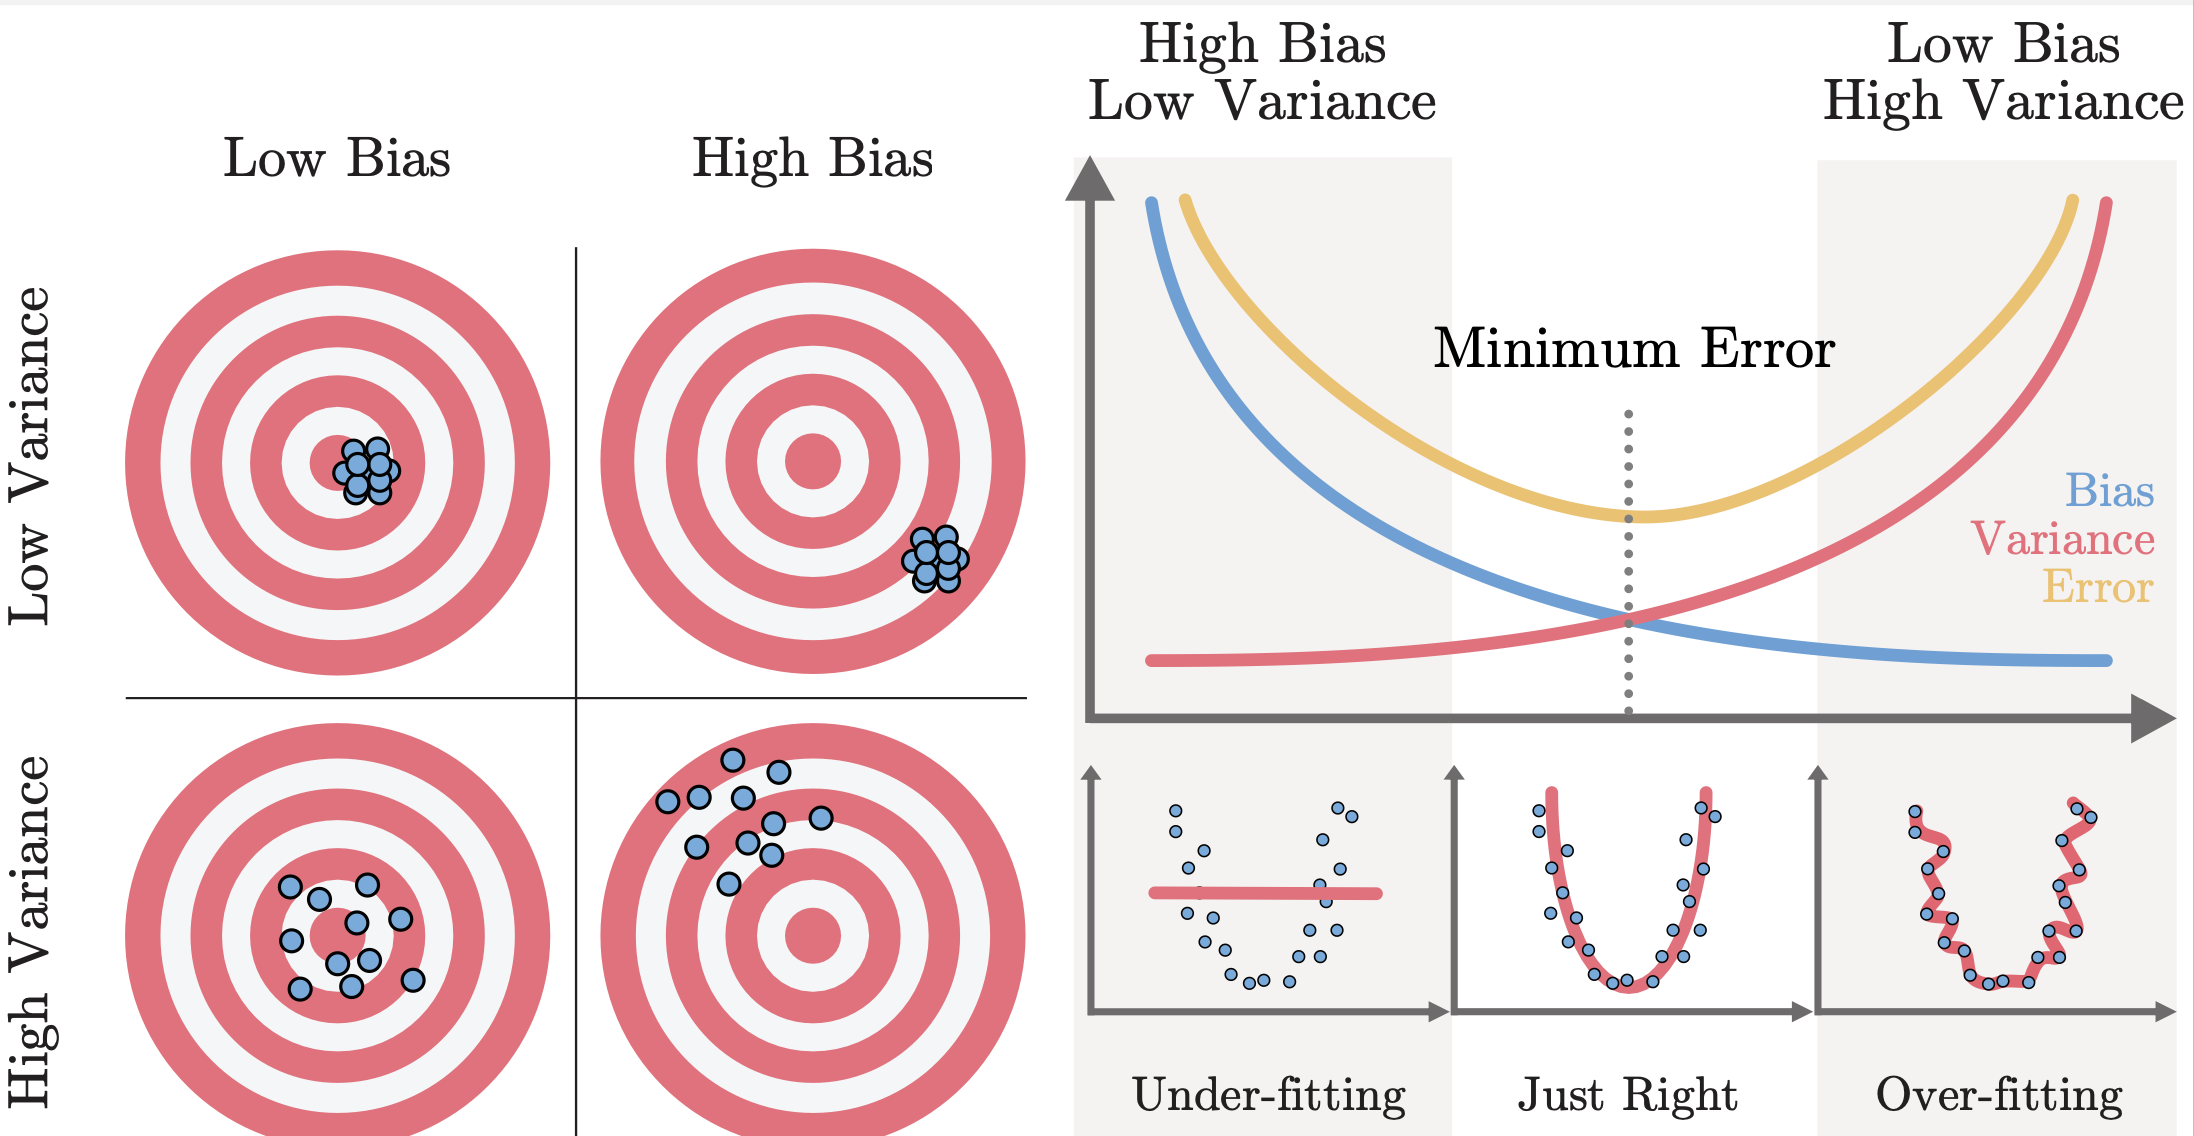
\includegraphics[width=0.65\textwidth]{cartoon1.png}
\caption{\label{fig:bias1}Diagrammatic representation of bias and variance and how we can over/under fit the model.}
\end{figure}




\section{Acknowledgements}


\appendix  
	
	\newpage
	\addcontentsline{toc}{section}{References}
	\bibliographystyle{utphys}
	\bibliography{ref.bib}
\end{document}